\documentclass[journal,12pt,twocolumn]{IEEEtran}

\usepackage{setspace}
\usepackage{gensymb}
\singlespacing
\usepackage[cmex10]{amsmath}

\usepackage{amsthm}

\usepackage{mathrsfs}
\usepackage{txfonts}
\usepackage{stfloats}
\usepackage{bm}
\usepackage{cite}
\usepackage{cases}
\usepackage{subfig}

\usepackage{longtable}
\usepackage{multirow}

\usepackage{enumitem}
\usepackage{mathtools}
\usepackage{steinmetz}
\usepackage{tikz}
\usepackage{circuitikz}
\usepackage{verbatim}
\usepackage{tfrupee}
\usepackage[breaklinks=true]{hyperref}
\usepackage{graphicx}
\usepackage{tkz-euclide}

\usetikzlibrary{calc,math}
\usepackage{listings}
    \usepackage{color}                                            %%
    \usepackage{array}                                            %%
    \usepackage{longtable}                                        %%
    \usepackage{calc}                                             %%
    \usepackage{multirow}                                         %%
    \usepackage{hhline}                                           %%
    \usepackage{ifthen}                                           %%
    \usepackage{lscape}     
\usepackage{multicol}
\usepackage{chngcntr}

\DeclareMathOperator*{\Res}{Res}

\renewcommand\thesection{\arabic{section}}
\renewcommand\thesubsection{\thesection.\arabic{subsection}}
\renewcommand\thesubsubsection{\thesubsection.\arabic{subsubsection}}

\renewcommand\thesectiondis{\arabic{section}}
\renewcommand\thesubsectiondis{\thesectiondis.\arabic{subsection}}
\renewcommand\thesubsubsectiondis{\thesubsectiondis.\arabic{subsubsection}}


\hyphenation{op-tical net-works semi-conduc-tor}
\def\inputGnumericTable{}                                 %%

\lstset{
%language=C,
frame=single, 
breaklines=true,
columns=fullflexible
}
\begin{document}


\newtheorem{theorem}{Theorem}[section]
\newtheorem{problem}{Problem}
\newtheorem{proposition}{Proposition}[section]
\newtheorem{lemma}{Lemma}[section]
\newtheorem{corollary}[theorem]{Corollary}
\newtheorem{example}{Example}[section]
\newtheorem{definition}[problem]{Definition}

\newcommand{\BEQA}{\begin{eqnarray}}
\newcommand{\EEQA}{\end{eqnarray}}
\newcommand{\define}{\stackrel{\triangle}{=}}
\bibliographystyle{IEEEtran}
\raggedbottom
\setlength{\parindent}{0pt}
\providecommand{\mbf}{\mathbf}
\providecommand{\pr}[1]{\ensuremath{\Pr\left(#1\right)}}
\providecommand{\qfunc}[1]{\ensuremath{Q\left(#1\right)}}
\providecommand{\sbrak}[1]{\ensuremath{{}\left[#1\right]}}
\providecommand{\lsbrak}[1]{\ensuremath{{}\left[#1\right.}}
\providecommand{\rsbrak}[1]{\ensuremath{{}\left.#1\right]}}
\providecommand{\brak}[1]{\ensuremath{\left(#1\right)}}
\providecommand{\lbrak}[1]{\ensuremath{\left(#1\right.}}
\providecommand{\rbrak}[1]{\ensuremath{\left.#1\right)}}
\providecommand{\cbrak}[1]{\ensuremath{\left\{#1\right\}}}
\providecommand{\lcbrak}[1]{\ensuremath{\left\{#1\right.}}
\providecommand{\rcbrak}[1]{\ensuremath{\left.#1\right\}}}
\theoremstyle{remark}
\newtheorem{rem}{Remark}
\newcommand{\sgn}{\mathop{\mathrm{sgn}}}
\providecommand{\abs}[1]{\left\vert#1\right\vert}
\providecommand{\res}[1]{\Res\displaylimits_{#1}} 
\providecommand{\norm}[1]{\left\lVert#1\right\rVert}
%\providecommand{\norm}[1]{\lVert#1\rVert}
\providecommand{\mtx}[1]{\mathbf{#1}}
\providecommand{\mean}[1]{E\left[ #1 \right]}
\providecommand{\fourier}{\overset{\mathcal{F}}{ \rightleftharpoons}}
%\providecommand{\hilbert}{\overset{\mathcal{H}}{ \rightleftharpoons}}
\providecommand{\system}{\overset{\mathcal{H}}{ \longleftrightarrow}}
	%\newcommand{\solution}[2]{\textbf{Solution:}{#1}}
\newcommand{\solution}{\noindent \textbf{Solution: }}
\newcommand{\cosec}{\,\text{cosec}\,}
\providecommand{\dec}[2]{\ensuremath{\overset{#1}{\underset{#2}{\gtrless}}}}
\newcommand{\myvec}[1]{\ensuremath{\begin{pmatrix}#1\end{pmatrix}}}
\newcommand{\mydet}[1]{\ensuremath{\begin{vmatrix}#1\end{vmatrix}}}
\numberwithin{equation}{subsection}
\makeatletter
\@addtoreset{figure}{problem}
\makeatother
\let\StandardTheFigure\thefigure
\let\vec\mathbf
\renewcommand{\thefigure}{\theproblem}
\def\putbox#1#2#3{\makebox[0in][l]{\makebox[#1][l]{}\raisebox{\baselineskip}[0in][0in]{\raisebox{#2}[0in][0in]{#3}}}}
     \def\rightbox#1{\makebox[0in][r]{#1}}
     \def\centbox#1{\makebox[0in]{#1}}
     \def\topbox#1{\raisebox{-\baselineskip}[0in][0in]{#1}}
     \def\midbox#1{\raisebox{-0.5\baselineskip}[0in][0in]{#1}}
\vspace{3cm}
\title{Assignment 5}
\author{Gautham Bellamkonda - CS20BTECH11017}
\maketitle
\newpage
\bigskip
\renewcommand{\thefigure}{\theenumi}
\renewcommand{\thetable}{\theenumi}
Download all python codes from 
\begin{lstlisting}
https://github.com/GauthamBellamkonda/AI1103/tree/main/Assignment5/Codes
\end{lstlisting}
and latex-tikz codes from 
\begin{lstlisting}
https://github.com/GauthamBellamkonda/AI1103/tree/main/Assignment5
\end{lstlisting}
\section{Problem (\textsc{Gate 2019 ST, Q43 Statistics Section})}
 Let $X$ be a random variable with uniform distribution on the interval $(-1, 1)$ and $Y=(X + 1)^2$. Then the probability density function $f(y)$ of $Y$, over the interval (0,4), is 
\begin{enumerate}
\item $\dfrac{3\sqrt{y}}{16}$ \\
\item $\dfrac{1}{4\sqrt{y}}$ \\
\item $\dfrac{1}{6\sqrt{y}}$ \\
\item $\dfrac{1}{\sqrt{y}}$ 
\end{enumerate}
\section{Solution}
We know that, since $Y = (X+1)^2$, 
\begin{align}
F_Y(y) = 0 \; \forall \; y < 0
\end{align}
Therefore, for $y\geq 0$, 
\begin{align}
F_Y(y) &= \pr{(x+1)^2 \leq y} \\
&= \pr{-\sqrt{y} - 1 \leq x \leq \sqrt{y} - 1 } \\
&= \pr{-\sqrt{y} - 1 \leq x \leq \sqrt{y} - 1 } \\
&= F_X(\sqrt{y} - 1) - F_X(-\sqrt{y} - 1) 
\label{eqn_}
\end{align}
Since $X$ is a uniform random variable in $(-1, 1)$,
\begin{align}
f_X(x) &= 
\begin{cases}
\frac{1}{2} & -1 < x < 1 \\
0 & \text{otherwise}
\end{cases}\\
F_X(x) &= 
\begin{cases}
0 & x \leq -1 \\
\frac{x}{2} + \frac{1}{2} & -1 < x < 1 \\
1 & x \geq 1
\end{cases}
\label{cdf_x}
\end{align}
Using \eqref{cdf_x} in \eqref{eqn_}, and using the fact that 
\begin{align}
-\sqrt{y}-1 \leq -1 \; \forall \; y \geq 0,
\end{align}
we get
\begin{align}
F_Y(y) &=  \begin{cases}
F_X(\sqrt{y} - 1) - 0 & y \geq 0\\
0 & y < 0
\end{cases} \\
&= \begin{cases}
0 & y < 0 \\
\frac{\sqrt{y}}{2}  & 0 \leq y \leq 4\\
1 & y > 4
\end{cases}
\end{align}
Therefore, 
\begin{align}
f_Y(y) &= \begin{cases}
\frac{1}{4\sqrt{y}}  & 0 \leq y \leq 4\\
0 & \text{otherwise}
\end{cases}
\end{align}
Therefore, \textbf{option 2} is correct. Fig. \ref{CDF_Y} shows a theoretical vs simulated plot of the PDF of random variable $Y$.
\begin{figure}[!hbt]
    \centering
	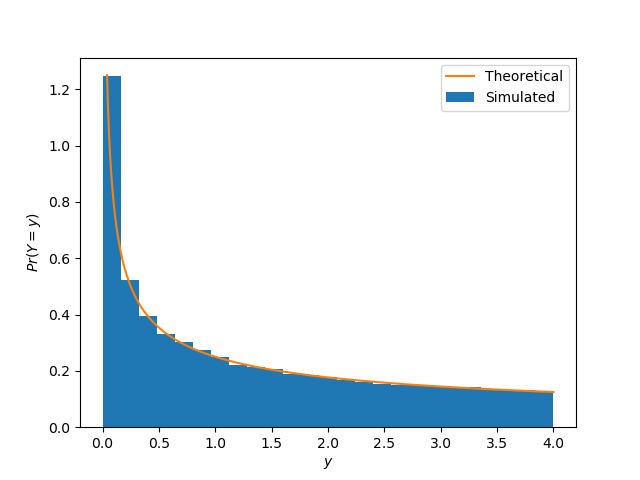
\includegraphics[width=\columnwidth]{./Figures/Figure_1.png}
    \caption{The PDF of $Y$}
    \label{CDF_Y}
\end{figure}
\end{document}